\documentclass[9pt,a4paper]{article}
\usepackage[T1]{fontenc}
\usepackage{times}
\usepackage{tikz}
\usepackage{ictamxs}
\usepackage{graphicx}
\usepackage{caption}
\usepackage{amsmath}
\usepackage{multicol}
\usepackage{indentfirst}
\usepackage{geometry}
\usepackage{natbib}
\usepackage{bm}

\bibliographystyle{abbrv}


\captionsetup[figure]{labelsep=period, name={Figure}, font=small}
\captionsetup[table]{labelsep=period, name={Table}, font=small}

\setlength{\textheight}{250mm}
\setlength{\topmargin}{-21mm}
\setlength{\textwidth}{16.5cm}
\setlength{\oddsidemargin}{-1mm}

\def\thefootnote{}
\begin{document}

\title{On the microstructure of buoyant emulsions}
%
\authors{
Nicolas Fintzi$^1 $, Jean-Lou Pierson$^1 $ \&\underline{ St\'ephane Popinet$^2$$^{\rm *}$}}
%
\footnotetext {\hskip -0.5cm\scriptsize $^{\rm *}$ Corresponding
author. E-mail: stephane.popinet@basilisk.fr}

\affiliations{
$^1$IFP Energies Nouvelles, Rond-point de l'echangeur de Solaize, 69360 Solaize\\
$^2$Sorbonne Universit\'e, Institut Jean le Rond d'Alembert, 4 place Jussieu, 75252 PARIS CEDEX 05, France
}
%

\maketitle


\begin{summary}
    Buoyancy-driven emulsions are encountered in many chemical engineering processes such as gravity separators, liquid-liquid extractors, etc. The usual engineering practice to model such facilities is to make use of the averaged Navier-Stokes equations and population balance equation. 
    However, these methods necessitate closure laws and a deep understanding of particle pair statistics.
    Therefore, in a multiscale strategy, we perform Direct Numerical Simulations (DNS) of tri-periodic monodisperse buoyant emulsions.
    In addition, to providing data for the closure terms appearing in the averaged models, tri-periodic simulations are of great interest to understand and describe the microstructure of the suspension. 
    In this work, we present a concise analysis of the microstructure by analyzing pairs particles properties, within the framework of the \textit{Nearest Particle Statistics} recently revisited by \cite{zhang2021ensemble}. 
\end{summary}

\section*{methodology}
\setlength{\parindent}{10pt}
To archive tri-periodic simulations, we used a cubic multigrid mesh,
inside which we initialized an array of 125 droplets subjects to buoyancy forces only. 
The Navier-Stokes equations are discretized with a centered scheme. 
The two-phase flow solver use the volume of fluid method.
The reconstruction of the interfaces is computed using Piecewise Linear Interface Calculation. 
Lastly, the surface forces are computed assuming a constant surface tension coefficient. 
Consequently, the solver compute the one-fluid formulation of the momentum and mass conservation equation for Newtonian fluid together with a transport equation for color function (not shown here). 
% It reads,
% \begin{equation}
%     \frac{\partial \rho \textbf{u}}{\partial t} +\bm{\nabla}\cdot(\rho \textbf{uu}) = \bm{\nabla} \cdot \bm{\sigma} + \rho \textbf{g} + \textbf{f}_\sigma \delta_S,
% \end{equation}
% \begin{equation}
%     \bm{\nabla} \cdot \textbf{u} = 0,
% \end{equation}
% where $\delta_S$ is the surface distribution function, $\textbf{f}_\sigma$ the surface force defined as the curvature times the surface tension coefficient along the normal of the droplet surface. 
% $\bm{\sigma} = -p \textbf{I} + \mu_f [\nabla \textbf{u}+ (\nabla \textbf{u})^T]$, with $p$ the pressure, is the Newtonian stress tensor and $\textbf{g}$ is the gravitational acceleration.
The main specificity of these simulations is the use of the \texttt{no-coalescence.h} header file.
This algorithm prevents numerical coalesce to occur. 
This enables us to study a specific population of droplets within time, in our case a monodisperse distribution of droplets.
Besides, we change the simulation reference frame by applying a constant acceleration on the whole domain so that the bulk velocity of the simulation remain null.
This way we can carry out DNS for an arbitrary amount of time while the bulk velocity remain null. 
In practice, we ran our simulations at least for 300 inertial time. 

\begin{table}[h!]
    \centering
    % 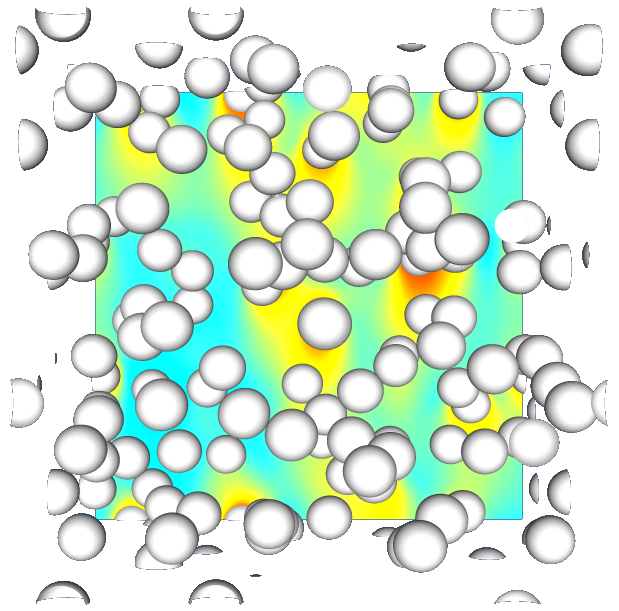
\includegraphics[width = 0.3\textwidth]{image/3D/P_PHI_5.png}

    \begin{tabular}{ccccccc}\hline
        $Ga$&$Bo$&$\phi$&$ \mu_r$&$\rho_r$\\ \hline\hline
        $5\rightarrow 100$&$0.2 \&  1$&$1\% \rightarrow 20\%$&$0.1 \& 1$&$1.111$\\ \hline
    \end{tabular}
    \vfill
    
    \caption{Dimensionless parameters investigated in this study.}
    \label{fig:pic}
\end{table}
The physical dimensionless parameters present in this problem are the following. 
The \textit{Galileo number}, $Ga$, which is the ratio of the buoyancy forces over
the viscosity forces.
The \textit{Bond number}, $Bo$, or the ratio between the buoyancy forces and surface tension forces.
The viscosity and density ratio are respectively noted, $\mu_r$ and $\rho_r$, (ratio of the dispersed phase over the continuous phase),
and the volume fraction of the dispersed phase is noted $\phi$. 
In this work we explored the range of parameters presented Table \ref{fig:pic} (right) which correspond to the industrial applications mentioned in summary.  

\section{Results}
\setlength{\parindent}{10pt}

In this study we present a statistical analysis of droplet interactions by using the recent \textit{Nearest Particle Statistics} framework proposed by \cite{zhang2021ensemble}. 
It consists in studying pairs interactions between particles and theirs nearest neighbor only. 
By sampling particles pairs properties from the DNS presented above, it is possible to reconstruct any nearest pair probability density functions. 
Presently, we focus on the averaged relative positions of the particles that we describe with the pair probability density, $P_\text{nst}(\textbf{r})$.
This PDF represents the probability of finding the center of mass of a droplet at the position \textbf{r} knowing its nearest neighbor's center of mass is located at $\textbf{r}=0$. 
Due to the possible physical implications, this PDF is also implicitly dependent on the dimensionless parameters, $Ga$, $Bo$, $\phi$, $\mu_r$ and $\rho_r$.
\begin{figure}
    \centering
    \begin{tikzpicture}
        \node (img1) at (0,1.7cm){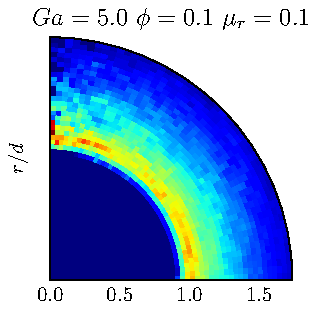
\includegraphics[width=3cm]{image/HOMOGENEOUS/fDrop/Pnst_mu_r_0_1_Ga_5_PHI_0_1}};
        \node (img2) at (3cm,1.7cm){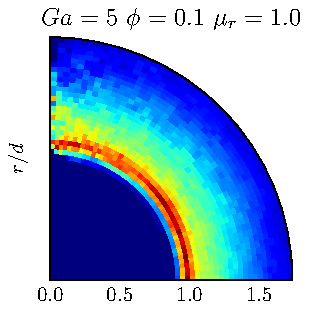
\includegraphics[width=3cm]{image/HOMOGENEOUS/fDrop/Pnst_mu_r_1_0_Ga_5_PHI_0_1}};
        \node (img3) at (0,-1.5cm){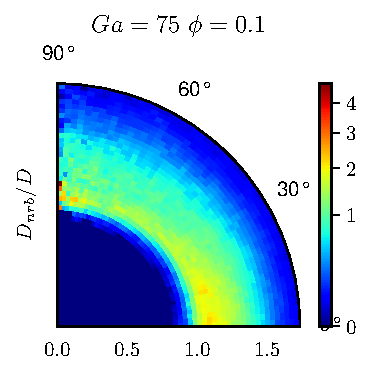
\includegraphics[width=3cm]{image/HOMOGENEOUS/fDrop/Pnst_mu_r_0_1_Ga_75_PHI_0_1}};
        \node (img4) at (3cm,-1.5cm){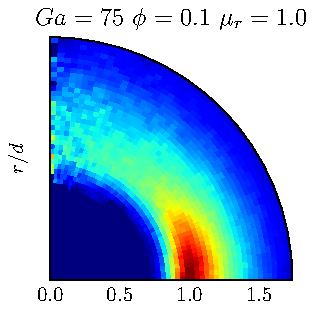
\includegraphics[width=3cm]{image/HOMOGENEOUS/fDrop/Pnst_mu_r_1_0_Ga_75_PHI_0_1}};
        \node (img5) at (7cm,0){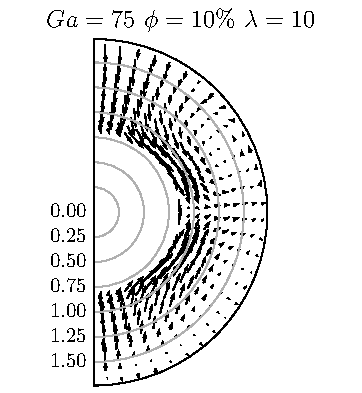
\includegraphics[width=5cm]{image/HOMOGENEOUS/fDrop/U_rel_l_10_Ga_75_PHI_10.pdf}};
        \node (img6) at (11.5cm,0){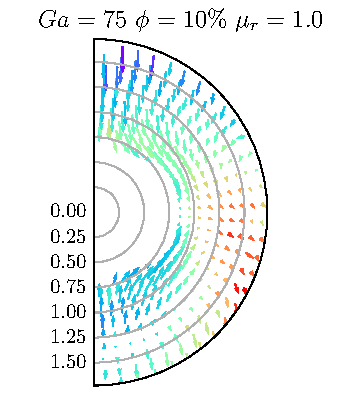
\includegraphics[width=5cm]{image/HOMOGENEOUS/fDrop/U_rel_l_1_Ga_75_PHI_10.pdf}};
        \draw (img1.south)node{(a)};
        \draw (img2.south)node{(b)};
        \draw (img3.south)node{(c)};
        \draw (img4.south)node{(d)};
        \draw (img5.south)node{(e)};
        \draw (img6.south)node{(f)};
    \end{tikzpicture}
    \caption{[(a), (b), (c), (d)] Probability density function of the nearest particle presence, $P_\text{nst}(\textbf{r})$ for two $Ga=5,75$ and two viscosity ratios.
    [(e), (f)] Averaged nearest particles relative velocity fields $\textbf{w}(\textbf{r},a)$ for respectively, $\mu_r = 0.1, 1$. 
     }
    \label{fig:icmf}
\end{figure}
Figure \ref{fig:icmf} displays the probability density $P_\text{nst}(\textbf{r})$ reconstructed from a DNS with highly viscous droplets ($\mu_r=0.1$, solid-like particles) and another one which has the same viscosity for both phases ($\mu_r=1$ bubble-like particles). 
Equally, two \textit{Galileo} numbers are displayed, a low inertial case $Ga=5$ and a high inertial case $Ga=75$. 
It is seen that the pair distribution function for $Ga = 5$ (panel (a) and (b)) is isotropic, while at higher $Ga$ (panel (c) and (d)) the distribution becomes denser on the sides. 
If we focus on the high inertial cases (panel (c) and (d)), we can observe that the pair distribution function is rather isotropic for $\mu_r = 0.1$ and align horizontally for $\mu_r = 1$. 
Additionally, a meticulous analysis of the radial probability density function $P_\text{nst}(|\textbf{r}|)$ (not shown here), leads us to the conclusions that particles are in average \textit{closer} with their nearest neighbor for emulsion with $\mu_r =1$ and high $Ga$. 
This latter observation can be interpreted as the presence of more packed clusters for high inertia and bubble-like particles \cite{zhang2023evolution}. 

In a second step we present the averaged relative velocity fields $\textbf{w}(\textbf{r},a)$.
It represents the averaged relative velocity between a particle and its nearest neighbor, knowing its nearest neighbor is located at the position $\textbf{r}$ with age $a$.
The age of interaction $a$, is the time from which the neighboring particle became the nearest particle, to the current sample time. 
Figure \ref{fig:icmf} panel (e) and (f), display these velocity fields, the color map represent the value of the age, from dark blue for $a = 0$ to dark red for the longest interactions. 
Following the color map and the vector fields, it can be stated that in average, the nearest neighboring particles approach from the vertical directions and leave through the sides of the particle of reference. 
In facts, the fields $\textbf{w}(\textbf{r},a)$ provides a quantitative averaged representation of what it is known as the Drafting Kissing Tumbling (DKT) mechanism.
Indeed, the relative motion seem similar to those predicted by DKT.
Although not obvious on these plots, the velocity field for $\mu_r = 1$ exhibit a clear stagnation zone on the sides of the test particle.
Consequently, all the neighboring particles end up being push to the sides at the end of their interaction, which clearly explain the shape of $P_\text{nst}(\textbf{r})$ shown Figure \ref{fig:icmf} panel (d). 
Regarding the case $\mu_r =0.1$, we observe a slightly different kinematic, indeed the particles doesn't necessarily end their interaction on the sides, which partly explain the different form of $P_\text{nst}(\textbf{r})$ compared wit the previous case.

\section{Discussion}
\vspace*{-10pt}


In this work, we carried out tri-periodic DNS of buoyant emulsion for a wide range of dimensionless parameters. 
We provided strong evidences on the nature of the pairwise interactions in buoyant emulsions by studying the probability density $P_\text{nst}(\textbf{r})$ and the relative conditional velocity field $\textbf{w}(\textbf{r},a)$. 
Within this framework  we could identify and quantify phenomena such as DKT mechanism and the shape of the microstructure. 
% We demonstrate that $\mu_r$ and $Ga$ has a strong impact on the spatial arrangement of the particles and also on their relative behavior. 
% To fully understand to interaction mechanism in an emulsion, these arguments must be completed by a dynamical analysis of the interactions between particles, however, for succinctness it will not be presented in this document.  
This study has been first motivated in the objective of building a coalescence kernel for the population balance equations. 
These coalescence models are based on the film drainage problems which assume a normal approach between droplets \cite{chesters1991modelling}.  
However, in light of Figure \ref{fig:icmf} (panel (e) and (f)), we showed that the interactions are more likely to happen tangentially rather than with a normal approach. 
We also demonstrated that $\mu_r$ and $Ga$ have a strong impact on the spatial arrangement of the particles and on their relative kinematic. 
For these reasons we conclude that there is a clear need to take in account these mechanisms, in the objective of building more accurate coalescence kernels. 
It could be done by considering a more sophisticated film drainage situation which would consider a relative velocity representative of $\textbf{w}(\textbf{r},a)$. 
This issue will be addressed in a future work.  



\bibliography{Bib/bib_bulles.bib}

\end{document}
